\documentclass[11pt,letterpaper,final,onecolumn]{article}
\usepackage[utf8]{inputenc}
\usepackage{amsmath}
\usepackage{amsfonts}
\usepackage{amssymb}
\usepackage{graphicx}
\graphicspath{{images/}}
\usepackage{cite}
\usepackage{enumerate}
\usepackage{url}
\usepackage{listings}
\usepackage[table]{xcolor}
\usepackage[UKenglish]{babel}% http://ctan.org/pkg/babel

\title{Peter Carl Fabergé}
\date{\today} 
\author{Max Sepulveda}

\begin{document}
\maketitle

\nocite{CalafateFloraChilena}
\nocite{ThePlantList}
\nocite{LeyendaCalafate}


\section{Peter Carl Fabergé}

Also known as Karl Gustavovich Fabergé (30th May 1846 - 24th September 1920), was a Russian jeweller best known for the famous Fabergé eggs made in the style of genuine Easter eggs, but using precious metals and gemstones rather than more mundane materials. He was the founder of the famous jewelry legacy House of Fabergé.

 \begin{figure}[hbt]
  \centering
   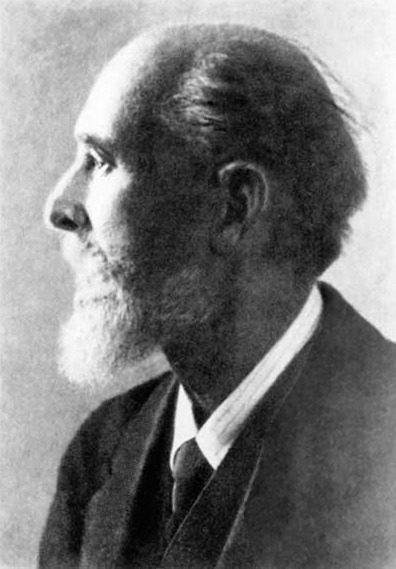
\includegraphics[scale=0.2]{Karl_Gustavovich_Faberge} 
   \caption{Peter Carl Fabergé}
   \label{fig:faberger}
 \end{figure}


\section{Another section}
\begin{itemize}
 \item Diosa de: $\dots\dots\dots\dots,\ \dots\dots\dots\dots,\ \dots\dots\dots\dots\ y\ \dots\dots\dots\dots$.
 \item Padres: $\dots\dots\dots\dots\ y\ \dots\dots\dots\dots$.
 \item Hijos: $\dots\dots\dots\dots,\ \dots\dots\dots\dots,\ \dots\dots\dots\dots,\ \dots\dots\dots\dots\ y\ \dots\dots\dots\dots$.
 \item Hera ayud a $\dots\dots\dots\dots$ en su viaje en busca del vellocino de oro.
\end{itemize}

\end{document}
